\documentclass[10pt,a4paper]{article}
\usepackage{amsmath,amssymb,amsthm,graphicx}
\usepackage{amsmath,amssymb,amsthm}
\usepackage{hyperref}
\usepackage{tikz,subcaption}
\usetikzlibrary{decorations.pathreplacing}
\newtheorem{theorem}{Theorem}
\newtheorem{problem}[theorem]{Problem}
\newtheorem{lemma}[theorem]{Lemma}
\newtheorem{corollary}[theorem]{Corollary}
\newcommand{\Order}{\mathrm O}
\newcommand{\OrderT}{\widetilde{\mathrm O}}
\newcommand{\OmegaT}{\widetilde\Omega}
\newcommand{\ThetaT}{\widetilde\Theta}
\newcommand{\polylog}{\operatorname{polylog}}
\newcommand{\poly}{\operatorname{poly}}
\newcommand{\given}{\,|\,}
\newcommand{\Exp}{\mathop{\mathbb E}}
\newcommand{\E}{\mathop{\mathbb E}}
\renewcommand{\Pr}{\mathbb P}
\title{Matching and vertex-cover lower bounds for short simple deletion streams via hidden augmented bi-index instances}
\author{Jacques Dark, Christian Konrad}
\date{doi:10.4230/LIPIcs.CCC.2020.30; CC BY 3.0 Unported}
\begin{document}
\maketitle
\noindent\textit{Editorial note.} Editable transcription of completeformallypublishedCCBY3.0Unported one-way deletionlowerbound theme. Nonexclusive nativev1 privateaid; publicselectedfiles onlycorrespondingformalmodels/Sections2–4 throughlastlowerboundcorollary. FullAugmentedBiIndex, bothgraphreductions anderror/parallelrunanalyses retained together; authorcalls themsame method, noobject/parameter/supportsplit. Alloriginalauthorconstants, inequalities andprobabilityexpressions preserved withoutmathematicalrepair ornewassumptions. AllnecessaryTikZ diagrams preservededitable; omittedintroFigure1 accounted byfigurecounter1. Originalglobaltheoremnumbers restored. Latervertexcoverupperboundsketch omitted. Noinput/include/assets. Allproduction/validationYupeng; rootownscompilation.\par\medskip
\noindent\textit{Allowed standard prerequisites (editorial).}\begin{itemize}
\item Randomized one-way AugmentedIndex lowerbound, bipartite matching/vertexcover and standardconcentration bounds. FullSection2 AugmentedBiIndex source-local reduction retained; standardAugmentedIndex theorem cited, completeSections3/4 graphreductions anderroranalysis included
\end{itemize}\medskip
\section*{One-way deletion communication and dynamic graph streams}
In our model, Alice holds a set of edges and sends a single message to Bob. Bob holds a set of edge deletions, which form a subset of Alice's edges, and needs to report a large matching or a small vertex cover in the graph spanned by the edges that are not deleted.
The lower bound constructions yield insertion-deletion streams of length $\Order(n^2)$ and do not involve multi-edges. The lower bounds therefore also hold for streaming algorithms that are designed for short input streams and simple graphs. Algorithms may output non-existing edges when they err.
A standard reduction shows that a lower bound on the size of Alice's message also constitutes a lower bound on the space requirements of an insertion-deletion streaming algorithm. The primary communication reductions and their stream consequences are retained together below.

\setcounter{section}{1}
\setcounter{figure}{1}
\section{Augmented Bi-Index} \label{sec:aug-bi-index}
In this section, we define the one-way two-party communication problem \textsf{Augmented Bi-Index} and prove a
lower bound on its communication complexity. 

\begin{problem}[\textsf{Augmented Bi-Index}]
    In an instance of {\em \textsf{Augmented Bi-Index}} {\em $\textsf{BInd}^{n,k}_\delta$} we have two players denoted Alice and Bob.
    Alice holds a binary matrix $A \in \lbrace 0,1 \rbrace^{n \times n}$. Bob holds indices $x, y \in [n-k]$ and the incomplete\footnote{We use $A_S$ to refer to the collection of entries indexed by the set $S$, so $A_S = (A_{i,j})_{(i,j)\in S}$.} binary matrix $A_{S(x,y)}$ where
    \[
        S(x,y) = \{ (i,j) \in [n]^2 \given (x \leq i < x + k) \text{ and } (y \leq j < y + k) \} \setminus \{ (x,y) \} \ .
    \]    
    Alice sends a single message $M$ to Bob who must output $A_{x, y}$ with probability at least $1-\delta$.
\end{problem}

Our lower bound proof consists of a reduction from the well-known \textsf{Augmented Index} problem, which is known to 
have large communication complexity.



%

\begin{problem}[\textsf{Augmented Index}]
    In an instance of {\em \textsf{Augmented Index}} {\em $\textsf{Ind}^{n}_\delta$} we have two players denoted Alice and Bob.
    Alice holds a binary vector $V \in \lbrace 0,1 \rbrace^n$. Bob holds an index $\ell \in [n]$ and the vector suffix $V_{>\ell} = (V_{\ell+1}, V_{\ell+2}, \cdots, V_n)$. 
    Alice sends a single message $M$ to Bob who must output $V_\ell$ with probability at least $1-\delta$.
\end{problem}

As a consequence of Lemma~13 in \cite{mnsw98}, we can see that this problem has linear communication complexity (see also Lemma~2 in \cite{bjkk04} for a more direct proof technique).

\begin{theorem}[e.g. \cite{mnsw98}]\label{thm:augind-lower}
    For $\delta < 1/3$, any randomised one-way communication protocol which solves $\textsf{Ind}^{n}_\delta$ must communicate $\Omega(n)$ bits.
\end{theorem}

%



%

We are now ready to prove our lower bound for \textsf{Augmented Bi-Index}.
\begin{theorem}\label{thm:bind-lower}
    For $\delta < 1/3$, any randomised one-way communication protocol which solves $\textsf{BInd}^{n,k}_\delta$ must communicate $\Omega((n-k)^2)$ bits.
\end{theorem}
\begin{proof}
    Let $\mathcal{P}$ be a communication protocol for $\textsf{BInd}^{n,k}_\delta$ that uses messages of length at most 
    $S(n, k)$ bits. We will show how $\mathcal{P}$ can be used to solve $\textsf{Ind}^{(n-k)^2}_\delta$ with the same message size.
    
    Let $V, \ell$ be any instance of $\textsf{Ind}^{(n-k)^2}_\delta$. Alice builds the matrix $A \in \{ 0, 1 \}^{n \times n}$ by placing the bits of $V$ in lexicographical order in the top-left $(n-k)$-by-$(n-k)$ region:
    \[
        A_{i,j} =   \begin{cases}
                        V_{j+(n-k)(i-1)} &\text{for } i,j \in [n-k]\\
                        0 &\text{otherwise}
                    \end{cases} \ .
    \]    
    This packing is illustrated in Figure~\ref{fig:aug-index}(a).
    
    Alice runs protocol $\mathcal{P}$ on $A$ and sends the resulting message $M$ to Bob.    
    Now, Bob has the message $M$, the index $\ell \in [(n-k)^2]$ and the suffix $V_{>\ell}$. Let $x, y \in [n-k]$ be the unique pair of integers such that $\ell = y + (n-k)(x-1)$. Observe that $A_{x,y} = V_\ell$.
    
    For Bob to be able to complete protocol $\mathcal{P}$ he needs to provide $A_{S(x,y)}$. Because of the way we packed the entries of $V$ onto $A$, the overlap between $V$ and $A_{S(x,y)}$ is a subset of the entries of $V_{>\ell}$ (see Figure~\ref{fig:aug-index}(b) for an illustration). Therefore Bob can complete the protocol and determine $A_{x,y} = V_\ell$ with probability at least $1-\delta$.    
    By Theorem~\ref{thm:augind-lower}, it must be that $S(n, k) = \Omega((n-k)^2)$.
\end{proof}

\begin{figure}
    \centering
    \hspace{1cm}
    \subcaptionbox{Example packing of the bits of $V$ into matrix $A$ with $n=9$ and $k=4$.}[0.4\textwidth]{
        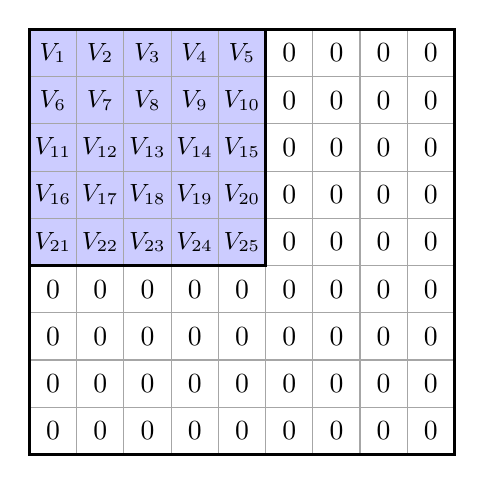
\begin{tikzpicture}[
            cell/.style={rectangle, draw=black!35!white, minimum size =6mm, inner sep=0mm}
        ]
            \fill[blue!20!white] (3mm, -3mm) rectangle (33mm, -33mm);
            \foreach \y in {1,...,5}
            {
                \foreach \x in {1,...,5}
                {                
                    \pgfmathtruncatemacro{\i}{int(int((\y-1)*5 + \x))}
                    \node[cell] at (6*\x mm, -6*\y mm) {\small $V_{\i}$};
                }
                \foreach \x in {6,...,9} \node[cell] at (6*\x mm, -6*\y mm) {$0$};
            }
            \foreach \y in {6,...,9}
            {
                \foreach \x in {1,...,9} \node[cell] at (6*\x mm, -6*\y mm) {$0$};
            }
            \draw[black, very thick] (3mm, -3mm) rectangle (57mm, -57mm);
            \draw[black, very thick] (3mm, -3mm) rectangle (33mm, -33mm);
        \end{tikzpicture}
    }
    \hspace{1cm}
    \subcaptionbox{Bob can construct the area $A_{S(x,y)}$ given $V_{>\ell}$, which is part of his input.}[0.4\textwidth]{
        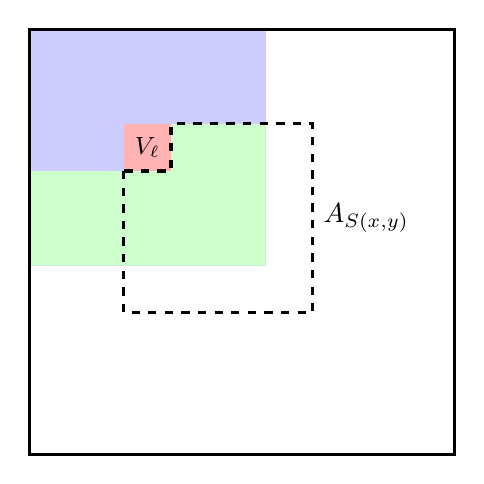
\begin{tikzpicture}[
            cell/.style={rectangle, minimum size =6mm, inner sep=0mm}
        ]
            \fill[blue!20!white] (3mm, -3mm) rectangle (33mm, -33mm);
            \node[cell, fill=red!30!white] at (18mm, -18mm) {\small $V_\ell$};
            \fill[green!20!white] (3mm, -21mm) -- (3mm, -33mm) -- (33mm, -33mm) -- (33mm, -15mm) -- (21mm, -15mm) -- (21mm, -21mm) -- (3mm, -21mm);
            \draw[very thick, dashed] (15mm, -21mm) -- (15mm, -39mm) -- (39mm, -39mm) -- node[right] {$A_{S(x,y)}$} (39mm, -15mm) -- (21mm, -15mm) -- (21mm, -21mm) -- (15mm, -21mm);
            \draw[black, very thick] (3mm, -3mm) rectangle (57mm, -57mm);
        \end{tikzpicture}
    }
    \caption{The construction of $A$ and $A_{S(x,y)}$ in Theorem~\ref{thm:bind-lower}.}
    \label{fig:aug-index}
\end{figure}

\section{Maximum Matching} \label{sec:matching}
Let $\mathbf{A}$ be a $C$-approximation insertion-deletion streaming algorithm for \textsf{Maximum Matching} that errs 
with probability at most $1/10$. We will now show that $\mathbf{A}$ can be used to solve $\textsf{BInd}^{n,k}_{\delta}$.

\subsection{Reduction}
Let $A \in \{0, 1\}^{n \times n}, x \in [n-k]$ and  $y \in [n-k]$ be an instance of $\textsf{BInd}^{n,k}_{\delta}$. 
Alice and Bob first sample a uniform random binary matrix $X \in \{0,1\}^{n \times n}$ 
and random permutations $\sigma_1, \sigma_2: [n] \rightarrow [n]$ from public randomness. Alice then computes matrix 
$A'$ which is obtained by first computing the entry-wise XOR of $A$ and $X$, denoted by $A \oplus X$, 
and then by permuting the rows and columns
of the resulting matrix by $\sigma_1$ and $\sigma_2$, respectively. Next, Alice interprets $A'$ as the incidence matrix
of a bipartite graph $G(A')$. Alice runs algorithm $\mathbf{A}$ on a random ordering of the edges of $G(A')$ and sends
the resulting memory state to Bob.

Next, Bob also computes the entry-wise XOR between the part of the matrix $A$ that he knows about, $A_{S(x,y)}$, and $X$, followed by applying
the permutations $\sigma_1$ and $\sigma_2$. In doing so, Bob knows the matrix entries of $A'$ at positions 
$(\sigma_1(i), \sigma_2(j))$
for every $(i,j) \in S(x,y)$. He can therefore compute the subset $E_S$ of the edges of $G(A')$ with

$$E_S = \{(\sigma_1(i),\sigma_2(j)) \in [n]^2 \ | \ (i,j) \in S(x,y) \mbox{ and } A'(\sigma_1(i),\sigma_2(j)) = 1  \} \ .$$

Furthermore, let $E_{diag} \subseteq E_S$ be the set of edges $(\sigma_1(i), \sigma_2(j))$ so that $(i,j)$ lies on the same
diagonal in $A$ as $(x,y)$, or, in other words, there exists an integer $1 \le q \le k-1$ such that $(x+q, y+q) = (i, j)$.
Then, let $E_{del} = E_S \setminus E_{diag}$.
Bob continues the execution of algorithm $\mathbf{A}$, as follows: for every edge $e \in E_{del}$, 
Bob introduces an edge deletion of $e$, in random order.

%
%
%
Let $M'$ be the matching returned by $\mathbf{A}$.
From $M'$ Bob computes the matching $M$ as follows: If $|M' \le 0.99 \frac{k}{2C}|$ then Bob sets $M = \varnothing$.
%
%
Otherwise, Bob sets $M$ to be a uniform random subset of $M'$ of size exactly $0.99 \frac{k}{2C}$.

\textbf{Parallel Executions.} Alice and Bob execute the previous process $\ell = 100 \cdot C$ times in parallel. Let $M^i$, $X^i$, 
$\sigma_1^i$ and $\sigma_2^i$ be $M$, $X$, $\sigma_1$ and $\sigma_2$ that are used in run $i$, respectively.
%
Let $Q_i$ be the indicator random variable that is $1$ iff $M^i$ contains the edge $(\sigma^i_1(x), \sigma^i_2(y))$. 
We also define $p = \sum_i Q_i$ to be the total number of times the edges $(\sigma^i_1(x), \sigma^i_2(y))$ are reported. 
Whenever the edge $(\sigma^i_1(x), \sigma^i_2(y))$ is reported, we interpret this to be a claim that $A_{x,y} = \neg X^i_{x,y}$. So depending on the value of $X^i_{x,y}$, this acts as a claim that $A_{x,y} = 0$ or $A_{x,y} = 1$. We define $p_0 = \sum_{i: Q_i = 1} X^i_{x, y}$ (which counts how often
$A_{x,y} = 0$ was claimed) and let $p_1 = p - p_0$ (the number of times $A_{x,y} = 1$ was claimed). Bob outputs $1$ as his estimator for $A_{x,y}$ if $p_1 \ge p_0$ 
and $0$ otherwise.


\subsection{Analysis}
Let $G$ be the bipartite graph with incidence matrix $A \oplus X$, and let 
$$F = \{ (i,j) \in S(x,y) \ | \ (A \oplus X)_{i,j} = 1 \mbox{ and } \nexists \ q \mbox{ s.t. } (i,j) = (x+q, y+q) \} \ .$$
Then the graph $G - F$ is isomorphic to the graph $G(A') - E_{del}$. In particular, 
$G(A') - E_{del}$ is obtained from $G - F$ by relabeling the vertex sets of the two bipartitions
using the permutations $\sigma_1$ and $\sigma_2$. 

We will first bound the maximum matching size in $G(A') - E_{del}$. To this end, we will bound the 
maximum matching size in $G - F$, which is easier to do:

\begin{lemma}\label{lem:matching-size}
 With probability $1-\frac{1}{k^{10}}$, the graph $G(A') - E_{del}$ is such that:
 $$0.99 \frac{k}{2} \le \mu(G(A') - E_{del}) \le 1.01 \frac{k}{2} + 2(n-k) \ ,$$
 where $\mu(G)$ denotes the \emph{matching number} of $G$, i.e., the size of a maximum matching.
\end{lemma}
\begin{proof}
 We will consider the graph $G - F$ instead, since it is isomorphic to $G(A') - E_{del}$ and has the same
 maximum matching size.
 
 First, observe that $G$ is a random bipartite graph where every edge is included with probability $\frac{1}{2}$.
 Let $U$ and $V$ denote the bipartitions in $G$, and consider the subsets $U' = [x, x+k)$ and $V' = [y, y+k)$.
 Observe that in the vertex induced subgraph $G[U' \cup V']$
 all edges are deleted in $F$ except those that connect 
 the vertices $x+i$ and $y+i$, for every $0 \le i \le k-1$. By a Chernoff bound, the number of edges and thus
 the maximum matching size in $G[U' \cup V']$ is bounded by:
 $$0.99 \cdot \frac{k}{2} \le \mu(G[U' \cup V']) \le 1.01 \cdot \frac{k}{2} \ , $$
 with probability $1 - \frac{1}{k^{10}}$.
 
 Observe that, with probability $1 - \frac{1}{k^{10}}$, the neighborhood $\Gamma(U')$ is such that 
 $$0.99 \cdot \frac{k}{2} \le |\Gamma(U')| \le 1.01 \cdot \frac{k}{2} + (n-k) \ .$$ 
 The set $U'$ can therefore be matched to at most $1.01 \cdot \frac{k}{2} + (n-k)$ vertices in $V$. 
 We thus obtain
 $$\mu(G - F) \le 1.01 \cdot \frac{k}{2} + 2(n-k) \ ,$$
 since we may also be able to match all $n-k$ vertices of $U \setminus U'$. 
\end{proof}


\begin{lemma}\label{lem:learn}
 Suppose that $M_i \neq \varnothing$. Then:
 \begin{eqnarray*}
\frac{0.99}{2C} - \frac{2(n - k)}{k} & \le & \Pr \left[ Q_i = 1 \right] \le \frac{0.99}{2C} \ .
%
 \end{eqnarray*}
 
%
\end{lemma}
\begin{proof}
 First, by construction of our reduction, since $M_i \neq \varnothing$ we have 
 $|M_i| = 0.99 \frac{k}{2C}$. 
 Let 
 $$U'_i = \sigma_1^i([x, x+k)) \mbox{ and } V'_i = \sigma_2^i([y, y+k)) \ .$$ 
 Let $\tilde{M}_i$ be the set of edges of $M_i$ connecting vertices in $U'_i$ to $V'_i$. Observe that there are
 $2(n-k)$ vertices in the graph outside the set $U'_i \cup V'_i$. We thus 
 have  
 $$|M_i| - 2(n-k) \le |\tilde{M}_i| \le |M_i|  \ .$$ 
 Next, since the permutations $\sigma^i_1, \sigma^i_2$ are chosen uniformly at random, any edge of $\tilde{M}_i$
 may have originated from any of the diagonal entries in $A_{S(x, y)}$. Hence, $\tilde{M}_i$ claims the bits
 of at least $|M_i| - 2(n-k)$ and at most $|M_i|$ uniform random positions in the diagonal of $A_{S(x, y)}$.
 Every entry in the diagonal of $A_{S(x,y)}$ is thus claimed with the same probability.
 Since the diagonal of $A_{S(x,y)}$ is of length $k$, this probability is at least
 $$ 
 \frac{|M_i| - 2(n-k)}{k} = \frac{0.99 \frac{k}{2C} - 2(n-k)}{k} = \frac{0.99}{2C} - \frac{2(n - k)}{k} \ ,
 $$
 and at most
 $$\frac{|M_i|}{k} = \frac{0.99 \frac{k}{2C}}{k} = \frac{0.99}{2C} \ .$$ 
\end{proof}



%
%

%
%
%
%
%
%
%
%
%
%
%
%




\begin{theorem}\label{thm:reduction} 
 Let $\mathbf{A}$ be a $n^{\epsilon}$-approximation insertion-deletion streaming algorithm 
 for \textsf{Maximum Matching} that errs with probability at most $1/10$ and uses space $s$. Then there exists a communication 
 protocol for $\textsf{BInd}^{n,n - \frac{1}{40} n^{1-\epsilon}}_{0.05}$ that communication $\Order(n^\epsilon \cdot s)$ bits.
\end{theorem}

\begin{proof}
Let $C = n^{\epsilon}$ and let $k = n - \frac{1}{40} n^{1-\epsilon}$.
 First, by Lemma~\ref{lem:matching-size}, with probability $1-\frac{1}{k^{10}}$, the graph 
 $G(A') - E_{del}$ contains a matching of size at least $0.99 k/ 2$. By a union bound, 
 the probability that this graph is of at least this size in each of the $\ell$ iterations  
 is at least $1 - \frac{\ell}{k^{10}}$. Suppose from now on that this event happens.

 Let $\ell_1$ be the number of times the algorithm $\mathbf{A}$ succeeds, and let $\ell_0$ be the number of times $\mathbf{A}$
 errs. Then, $\ell = \ell_0 + \ell_1$. Whenever $\mathbf{A}$ succeeds, since $\mathbf{A}$ is a $C$-approximation
 algorithm, the matching $M'_i$ is of size $0.99 \frac{k}{2C}$, which further implies that $M_i$ is of size exactly
 $0.99 \frac{k}{2C}$. Since the algorithm must return a correct matching, every time we have a claim (i.e. $Q_i = 1$), the claimed bit value must be correct. Thus, by Lemma~\ref{lem:learn}, we get a correct claim on $A_{x,y}$ with probability at least 
 \begin{eqnarray*}
  \frac{0.99}{2C} - \frac{2(n - k)}{k} & = & \frac{0.99}{2n^{\epsilon}} - \frac{2(\frac{1}{40} n^{1-\epsilon})}{n - \frac{1}{40} n^{1-\epsilon}} \ge  \frac{0.99}{2n^{\epsilon}} - \frac{\frac{1}{40} n^{1-\epsilon}}{n} = \frac{0.99}{2n^{\epsilon}} - \frac{1}{40n^{\epsilon}} \ge \frac{2}{5 n^\epsilon}   \ , \label{eqn:018}
 \end{eqnarray*}
where we used the inequality $\frac{2x}{y-x} \ge \frac{x}{y}$, which holds for every $y > x$. 
We thus expect to see the correct bit claimed at least $\ell_1 \cdot \frac{2}{5 n^\epsilon}$ times in total.
On the other hand, incorrect claims of the bit value can only occur when the algorithm errs. In the worst case, $\mathbf{A}$ 
will make as many false claims as possible - so we assume the algorithm never results in $M_i = \emptyset$ when it errs. 
Lemma~\ref{lem:learn} also allows us to bound the probability of an incorrect claim for this bad algorithm by $\frac{0.99}{2n^\epsilon}$. We thus expect to see the wrong bit value claimed at most $\ell_0 \cdot \frac{0.99}{2C} \le \frac{\ell_0}{2n^\epsilon}$ times.
 
 Recall that $\ell = 100 n^\epsilon$. Then, by standard concentration bounds, the probability that 
 $\ell_0 \ge 2 \cdot \frac{\ell}{10}$ is at most $\frac{1}{100}$ (recall that the error probability of $\mathbf{A}$ 
 is at most $\frac{1}{10}$). Suppose now that $\ell_0 \le \frac{1}{5} \ell$ holds, which also implies that $\ell_1 \ge \frac{4}{5} \ell$.
 We thus expect to learn the correct bit at least 
 $$\frac{4}{5} 100 n^{\epsilon} \cdot \frac{2}{5 n^\epsilon} = 32$$
 times, and using a Chernoff bound, it can be seen that the probability that we learn the correct bit less than 
 $21$ times is at most $0.02$. 
 Similarly, we expect to learn the incorrect bit at most 
 $$\frac{1}{5} 100 n^{\epsilon} \cdot \frac{1}{2n^\epsilon} = 10$$
 times, and by a Chernoff bound, it can be seen that the probability that we learn the incorrect bit at least $20$ times 
 is at most $ 0.01$. Our algorithm therefore succeeds if all these events happen. Taking a union bound
 over all failure probabilities that occurred in this proof, we see that our algorithm succeeds with probability
 $$1 - \frac{100n^{\epsilon}}{k^{10}} - 0.01 - 0.02 - 0.01 \ge 0.95 \ .$$
\end{proof}

Since by Theorem~\ref{thm:bind-lower}, $\textsf{BInd}^{n,n - \frac{1}{40} n^{1-\epsilon}}_{0.05}$ has randomized one-way 
communication complexity $\Omega(n^{2-2\epsilon})$, by Theorem~\ref{thm:reduction} we obtain our main result of this section:
%
\begin{corollary}
 Every insertion-deletion $n^\epsilon$-approximation streaming algorithm  
 for \textsf{Maximum Matching} that errs with probability at most $\frac{1}{10}$ requires space $\Omega(n^{2-3\epsilon})$.
\end{corollary}




\section{Minimum Vertex Cover} \label{sec:vertex-cover}
Let $\mathbf{B}$ be a $C$-approximation insertion-deletion streaming algorithm for \textsf{Minimum Vertex Cover} that succeeds with
probability $1 - 1/400$. Similar to the previous section, we will now show how $\mathbf{B}$ can be used to solve $\textsf{BInd}^{n,k}_{\delta}$.

\subsection{Reduction}
Let $A \in \{0, 1\}^{n \times n}, x \in [n-k]$ and  $y \in [n-k]$ be an instance of $\textsf{BInd}^{n,k}_{\delta}$. 
The reduction for \textsf{Minimum Vertex Cover} is very similar to the reduction for \textsf{Maximum Matching} presented 
in the previous section. Alice's behaviour is in fact identical: 

First, Alice and Bob sample a uniform random binary matrix $X \in \{0,1\}^{n \times n}$ and random permutations 
$\sigma_1, \sigma_2: [n] \rightarrow [n]$ from public randomness. 
Alice then computes matrix $A'$ which is obtained by first computing $A \oplus X$
and then  permuting the rows and then the columns of the resulting matrix by $\sigma_1$ and $\sigma_2$, respectively. 
Alice interprets $A'$ as the incidence matrix of a bipartite graph $G(A')$. Alice then runs algorithm $\mathbf{B}$ 
on a random ordering of the edges of $G(A')$ and sends the resulting memory state to Bob.

Next, Bob also computes the entry-wise XOR between the part of the matrix $A$ that he knows about and $X$, followed by applying
the permutations $\sigma_1$ and $\sigma_2$. In doing so, Bob knows the matrix entries of $A'$ at positions 
$(\sigma_1(i), \sigma_2(j))$
for every $(i,j) \in S(x,y)$. He can therefore compute the subset $E_S$ of the edges of $G(A')$ with

$$E_S = \{(\sigma_1(i),\sigma_2(j)) \in [n]^2 \ | \ (i,j) \in S(x,y) \mbox{ and } A'(\sigma_1(i),\sigma_2(j)) = 1  \} \ .$$

Next, Bob continues the execution of $\mathbf{B}$ and introduces deletions {\em for all edges in $E_S$} in random order. 
Observe that this 
step is different to the reduction for \textsf{Maximum Matching}. Let $I$ be the vertex cover produced by $\mathbf{B}$.
%

\textbf{Parallel Executions.} Alice and Bob run the procedure above $40$ times in parallel. Denote by $I^i$, $X^i$, $E^i_S$,
$A'^i$, $\sigma_1^i$, and $\sigma_2^i$ the variables $I, X, E_S, A', \sigma_1$ and $\sigma_2$ used in iteration $i$.  
Furthermore, let $Q_i$ be 
the indicator variable that is $1$ iff $\{ \sigma^i_1(x), \sigma^i_2(y) \} \cap I_i \neq \varnothing$,
i.e., the potential edge $(\sigma^i_1(x), \sigma^i_2(y))$ is covered by the vertex cover. 

If there exists a run $j$ with $Q_j = 0$, then Bob predicts $A_{x,y} = X_{x,y}$ (if there are multiple such runs
then Bob breaks ties arbitrarily). Otherwise, Bob returns \texttt{fail} and the algorithm errs.

\subsection{Analysis}
%
%
%
%
%
%

The first lemma applies to every parallel run $j$. For simplicity of notation, we will omit
the superscripts that indicate the parallel run in our random variables.

We first show an upper bound on the size of a minimum vertex cover in $G(A') - E_S$.

\begin{lemma}\label{lem:vc-size}
 The size of a minimum vertex cover in $G(A') - E_S$ is at most $2(n-k) + 1$.
\end{lemma}
\begin{proof}
Let $U, V$ be the bipartitions of the graph $G(A') - E_S$, let $U' = \{\sigma_1(a) \ : \ a \in [x, x+k) \}$ and let
$V' = \{\sigma_2(b) \ : \ b \in [y, y+k) \}$. Observe that $(G(A') - E_S)[U' \cup V']$ 
contains at most one edge: The potential edge between $\sigma_1(x)$ and $\sigma_2(y)$. A valid vertex cover 
of $G(A') - E_S$ is therefore $(U \setminus U') \cup (V \setminus V') + \sigma_1(x)$,
which is of size $2(n-k) + 1$.
\end{proof}

Next, we prove the key property of our reduction: We show that if $A'_{\sigma_1(x), \sigma_2(y)} = 0$ (or equivalently, 
$A_{x,y} \oplus X_{x,y} = 0$)
then neither $\sigma_1(x)$ nor $\sigma_2(y)$ is in the output vertex cover with large probability.

\begin{lemma} \label{lem:covered}
 Assume that algorithm $\mathbf{B}$ does not err in run $j$. Suppose that 
 $A'^j_{\sigma^j_1(x), \sigma^j_2(y)} = 0$. Then the probability that $Q_j = 1$ is at most 
 $$\frac{3 C \cdot (2(n-k) + 1)}{k} \ .$$
\end{lemma}
\begin{proof}
 Consider the set $D  = \{ (\sigma^j_1(x + i), \sigma^j_2(y+i)) \ | \ 0 \le i \le k-1 \}$, i.e., the positions of the diagonal
 of $S(x,y) \cup \{x, y\}$ permuted by $\sigma^j_1$ and $\sigma^j_2$. Then, since $A'^j$ is a uniform random matrix, with probability
 at least $1-\frac{1}{k^{10}}$, the ``permuted diagonal'' $A'^j_{D}$ contains at least $0.99 k/ 2$ entries with value $0$,
 or, in other words, graph $G(A'^j) - E^j_S$ contains at least $0.99 k/ 2$ non-edges in the positions of the permuted diagonal $D$.
 By Lemma~\ref{lem:vc-size}, the size of a minimum vertex cover in $G(A'^{j}) - E^{j}_S$ is at most $2(n-k) + 1$, and since
 $\mathbf{B}$ has an approximation factor of $C$, the  vertex cover $I_j$ is of size at most $C \cdot (2(n-k) + 1)$. Hence, 
 at most $C \cdot (2(n-k) + 1)$ non-edges in $D$ can be covered in $I_j$. However, since the permutations are random, the 
 probability that the non-edge $(\sigma^j_1(x), \sigma^j_2(y))$
 is covered, which is identical to the event $Q_j = 1$, is therefore at most 
 $$\frac{C \cdot (2(n-k) + 1)}{0.99 k/ 2} \le \frac{3 C \cdot (2(n-k) + 1)}{k} \ .$$
\end{proof}



\begin{theorem} \label{thm:vc-reduction}
 Let $\mathbf{B}$ be a $n^{\epsilon}$-approximation 
 insertion-deletion streaming algorithm for \textsf{Minimum Vertex Cover} that uses space $s$ and errs with probability 
 at most $1/400$. Then, there exists a communication protocol for $\textsf{BInd}^{n,n - \frac{1}{20}n^{1-\epsilon}}_{\frac{1}{3}}$ 
 that communicates $\Order(s)$ bits.
\end{theorem}

\begin{proof}
Let $k = n - \frac{1}{40} n^{1-\epsilon}$ and let $C= n^{\epsilon}$.
 Consider the reduction given in the previous subsection. First, observe that since $\mathbf{B}$ errs with probability
 at most $1/400$, by the union bound the probability that $\mathbf{B}$ errs at least once in the $40$ parallel executions of our
 reduction is at most $\frac{1}{10}$. We assume from now on that the algorithm never errs.
 
 Observe that the matrices $A'^j$ are random matrices. Hence, 
%
%
 the probability that there exists at least one run $i$ with $A'^i_{\sigma^i_1(x), \sigma^i_2(y)} = 0$ is at least 
 $1 - (\frac{1}{2})^{40}$. Suppose that this event happens. Let run $i$ be so that $A'^i_{\sigma^i_1(x), \sigma^i_2(y)} = 0$.
 Then, by Lemma~\ref{lem:covered}, the probability that the non-edge $(\sigma^i_1(x), \sigma^i_2(y))$ is covered by $I_i$,
 or in other words, the probability that $Q_i = 1$, is at most 
 
 $$\frac{3 C \cdot (2(n-k) + 1)}{k} = \frac{3n^{\epsilon} \cdot (\frac{1}{20} n^{1-\epsilon} + 1) }{n - \frac{1}{40}n^{1-\epsilon}} = 
 \frac{\frac{3}{20}n + 3n^{\epsilon}}{n - \frac{1}{40}n^{1-\epsilon}} = \frac{3}{20} + o(1) \ . $$  
 
 Observe that whenever $Q_i = 0$, the algorithm outputs $X^i_{x,y}$ as a predictor for $A_{x,y}$. Since the algorithm $\mathbf{B}$ 
 does not err, we have $A_{x,y} \oplus X^i_{x,y} = 0$. This implies that $A_{x,y} = X^i_{x,y}$, which establishes correctness.
 
 Last, we need to bound the error probability of our algorithm. First, the probability that at least one of the $40$ runs 
 fails is at most $\frac{1}{10}$. Next, the probability that none of the runs are such that $A'^j_{\sigma^j_1(x), \sigma^j_2(y)} = 0$
 is at most $(\frac{1}{2})^{40}$. Furthermore, the probability that $Q_i = 1$ when $A'^i_{\sigma^i_1(x), \sigma^i_2(y)} = 0$ is at 
 most $\frac{3}{20} + o(1)$. Applying the union bound, we see that the overall error probability of our algorithm is at most
 $$\frac{1}{10}+ (\frac{1}{2})^{40} + \frac{3}{20} + o(1) \le \frac{1}{3} \ , $$
 for large enough $n$. 
\end{proof}
Since by Theorem~\ref{thm:bind-lower}, $\textsf{BInd}^{n,n - \frac{1}{40}n^{1-\epsilon}}_{\frac{1}{3}}$ has a 
communication complexity of $\Omega(n^{2-2\epsilon})$, we
obtain the following result:
\begin{corollary}
 Every insertion-deletion $n^\epsilon$-approximation streaming algorithm for \textsf{Minimum Vertex Cover} with error probability 
 at most $\frac{1}{400}$ requires space $\Omega(n^{2-2\epsilon})$.
\end{corollary}

\begin{thebibliography}{99}
\bibitem{bjkk04}
Bar-Yossef, Z., Jayram, T.S., Krauthgamer, R., Kumar, R.: The sketching
  complexity of pattern matching. In: Approximation, Randomization, and
  Combinatorial Optimization. Algorithms and Techniques, pp. 261--272. Springer
  (2004)

\bibitem{mnsw98}
Miltersen, P.B., Nisan, N., Safra, S., Wigderson, A.: On data structures and
  asymmetric communication complexity. Journal of Computer and System Sciences
  57(1),  37--49 (1998)

\end{thebibliography}
\end{document}
